\documentclass[tikz]{standalone}
\usetikzlibrary{fit}

\begin{document}
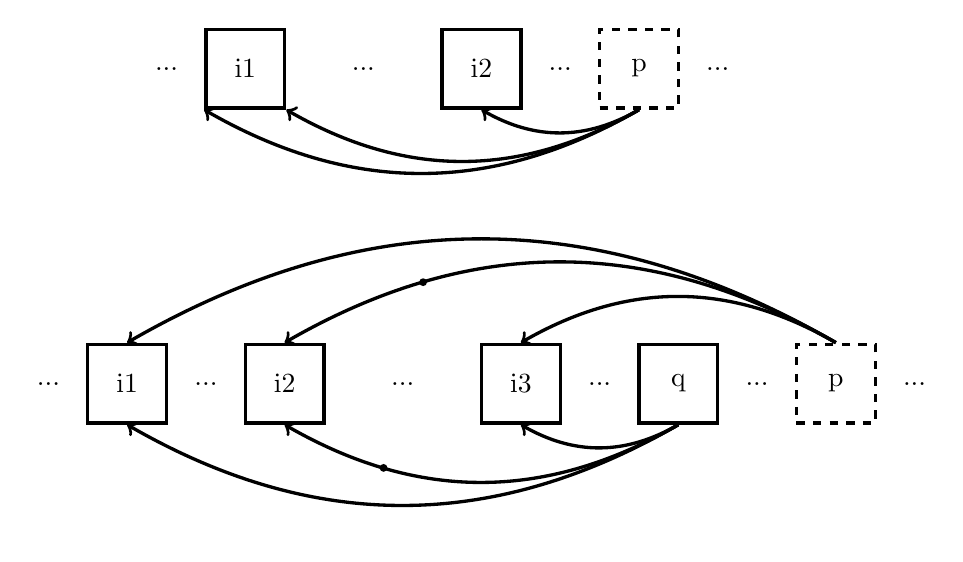
\begin{tikzpicture}[
    very thick,
    mignode/.style={
        rectangle,
        draw,
        inner sep=0pt,
        minimum size=1cm,
    },
    circ/.style={
        circle,
        fill,
        inner sep=1pt,
    },
]

\node at (0,0) {...};
\node[mignode] (i1) at (1,0) {i1};
\node at (2.5,0) {...};
\node[mignode] (i2) at (4,0) {i2};
\node at (5,0) {...};
\node[mignode, dashed] (p) at (6,0) {p};
\node at (7,0) {...};

\draw[->] (p.south) to[bend left] (i2.south);
\draw[->] (p.south) to[bend left] (i1.south east);
\draw[->] (p.south) to[bend left] (i1.south west);

\begin{scope}[xshift=-1.5cm,yshift=-4cm]
    \node at (0,0) {...};
    \node[mignode] (ch1) at (1,0) {i1};
    \node at (2,0) {...};
    \node[mignode] (ch2) at (3,0) {i2};
    \node at (4.5,0) {...};
    \node[mignode] (ch3) at (6,0) {i3};
    \node at (7,0) {...};
    \node[mignode] (q)   at (8,0) {q};
    \node at (9,0) {...};
    \node[mignode,dashed] (p)   at (10,0) {p};
    \node at (11,0) {...};

    \draw[->] (q.south) to[bend left] (ch3.south);
    \draw[->] (q.south) to[bend left] node[near end, circ]{}(ch2.south);
    \draw[->] (q.south) to[bend left] (ch1.south);

    \draw[->] (p.north) to[bend right] (ch3.north);
    \draw[->] (p.north) to[bend right] node[near end, circ]{}(ch2.north);
    \draw[->] (p.north) to[bend right] (ch1.north);

\end{scope}

\end{tikzpicture}
\end{document}